% Options for packages loaded elsewhere
\PassOptionsToPackage{unicode}{hyperref}
\PassOptionsToPackage{hyphens}{url}
%
\documentclass[
  11pt,
]{article}
\usepackage{amsmath,amssymb}
\usepackage{iftex}
\ifPDFTeX
  \usepackage[T1]{fontenc}
  \usepackage[utf8]{inputenc}
  \usepackage{textcomp} % provide euro and other symbols
\else % if luatex or xetex
  \usepackage{unicode-math} % this also loads fontspec
  \defaultfontfeatures{Scale=MatchLowercase}
  \defaultfontfeatures[\rmfamily]{Ligatures=TeX,Scale=1}
\fi
\usepackage{lmodern}
\ifPDFTeX\else
  % xetex/luatex font selection
    \setmainfont[]{DejaVu Sans}
\fi
% Use upquote if available, for straight quotes in verbatim environments
\IfFileExists{upquote.sty}{\usepackage{upquote}}{}
\IfFileExists{microtype.sty}{% use microtype if available
  \usepackage[]{microtype}
  \UseMicrotypeSet[protrusion]{basicmath} % disable protrusion for tt fonts
}{}
\makeatletter
\@ifundefined{KOMAClassName}{% if non-KOMA class
  \IfFileExists{parskip.sty}{%
    \usepackage{parskip}
  }{% else
    \setlength{\parindent}{0pt}
    \setlength{\parskip}{6pt plus 2pt minus 1pt}}
}{% if KOMA class
  \KOMAoptions{parskip=half}}
\makeatother
\usepackage{xcolor}
\usepackage[margin=2.5cm]{geometry}
\usepackage{color}
\usepackage{fancyvrb}
\newcommand{\VerbBar}{|}
\newcommand{\VERB}{\Verb[commandchars=\\\{\}]}
\DefineVerbatimEnvironment{Highlighting}{Verbatim}{commandchars=\\\{\}}
% Add ',fontsize=\small' for more characters per line
\usepackage{framed}
\definecolor{shadecolor}{RGB}{248,248,248}
\newenvironment{Shaded}{\begin{snugshade}}{\end{snugshade}}
\newcommand{\AlertTok}[1]{\textcolor[rgb]{0.94,0.16,0.16}{#1}}
\newcommand{\AnnotationTok}[1]{\textcolor[rgb]{0.56,0.35,0.01}{\textbf{\textit{#1}}}}
\newcommand{\AttributeTok}[1]{\textcolor[rgb]{0.13,0.29,0.53}{#1}}
\newcommand{\BaseNTok}[1]{\textcolor[rgb]{0.00,0.00,0.81}{#1}}
\newcommand{\BuiltInTok}[1]{#1}
\newcommand{\CharTok}[1]{\textcolor[rgb]{0.31,0.60,0.02}{#1}}
\newcommand{\CommentTok}[1]{\textcolor[rgb]{0.56,0.35,0.01}{\textit{#1}}}
\newcommand{\CommentVarTok}[1]{\textcolor[rgb]{0.56,0.35,0.01}{\textbf{\textit{#1}}}}
\newcommand{\ConstantTok}[1]{\textcolor[rgb]{0.56,0.35,0.01}{#1}}
\newcommand{\ControlFlowTok}[1]{\textcolor[rgb]{0.13,0.29,0.53}{\textbf{#1}}}
\newcommand{\DataTypeTok}[1]{\textcolor[rgb]{0.13,0.29,0.53}{#1}}
\newcommand{\DecValTok}[1]{\textcolor[rgb]{0.00,0.00,0.81}{#1}}
\newcommand{\DocumentationTok}[1]{\textcolor[rgb]{0.56,0.35,0.01}{\textbf{\textit{#1}}}}
\newcommand{\ErrorTok}[1]{\textcolor[rgb]{0.64,0.00,0.00}{\textbf{#1}}}
\newcommand{\ExtensionTok}[1]{#1}
\newcommand{\FloatTok}[1]{\textcolor[rgb]{0.00,0.00,0.81}{#1}}
\newcommand{\FunctionTok}[1]{\textcolor[rgb]{0.13,0.29,0.53}{\textbf{#1}}}
\newcommand{\ImportTok}[1]{#1}
\newcommand{\InformationTok}[1]{\textcolor[rgb]{0.56,0.35,0.01}{\textbf{\textit{#1}}}}
\newcommand{\KeywordTok}[1]{\textcolor[rgb]{0.13,0.29,0.53}{\textbf{#1}}}
\newcommand{\NormalTok}[1]{#1}
\newcommand{\OperatorTok}[1]{\textcolor[rgb]{0.81,0.36,0.00}{\textbf{#1}}}
\newcommand{\OtherTok}[1]{\textcolor[rgb]{0.56,0.35,0.01}{#1}}
\newcommand{\PreprocessorTok}[1]{\textcolor[rgb]{0.56,0.35,0.01}{\textit{#1}}}
\newcommand{\RegionMarkerTok}[1]{#1}
\newcommand{\SpecialCharTok}[1]{\textcolor[rgb]{0.81,0.36,0.00}{\textbf{#1}}}
\newcommand{\SpecialStringTok}[1]{\textcolor[rgb]{0.31,0.60,0.02}{#1}}
\newcommand{\StringTok}[1]{\textcolor[rgb]{0.31,0.60,0.02}{#1}}
\newcommand{\VariableTok}[1]{\textcolor[rgb]{0.00,0.00,0.00}{#1}}
\newcommand{\VerbatimStringTok}[1]{\textcolor[rgb]{0.31,0.60,0.02}{#1}}
\newcommand{\WarningTok}[1]{\textcolor[rgb]{0.56,0.35,0.01}{\textbf{\textit{#1}}}}
\usepackage{graphicx}
\makeatletter
\newsavebox\pandoc@box
\newcommand*\pandocbounded[1]{% scales image to fit in text height/width
  \sbox\pandoc@box{#1}%
  \Gscale@div\@tempa{\textheight}{\dimexpr\ht\pandoc@box+\dp\pandoc@box\relax}%
  \Gscale@div\@tempb{\linewidth}{\wd\pandoc@box}%
  \ifdim\@tempb\p@<\@tempa\p@\let\@tempa\@tempb\fi% select the smaller of both
  \ifdim\@tempa\p@<\p@\scalebox{\@tempa}{\usebox\pandoc@box}%
  \else\usebox{\pandoc@box}%
  \fi%
}
% Set default figure placement to htbp
\def\fps@figure{htbp}
\makeatother
\setlength{\emergencystretch}{3em} % prevent overfull lines
\providecommand{\tightlist}{%
  \setlength{\itemsep}{0pt}\setlength{\parskip}{0pt}}
\setcounter{secnumdepth}{5}
\ifLuaTeX
\usepackage[bidi=basic]{babel}
\else
\usepackage[bidi=default]{babel}
\fi
\babelprovide[main,import]{polish}
\ifPDFTeX
\else
\babelfont{rm}[]{DejaVu Sans}
\fi
% get rid of language-specific shorthands (see #6817):
\let\LanguageShortHands\languageshorthands
\def\languageshorthands#1{}
\usepackage{bookmark}
\IfFileExists{xurl.sty}{\usepackage{xurl}}{} % add URL line breaks if available
\urlstyle{same}
\hypersetup{
  pdftitle={Analiza zanieczyszczenia powietrza w Polsce},
  pdfauthor={Miriam Nieslona, Piotr Geremek, Bartosz Kurzyński, Jakub Kołpaczyński, Stanisław Kolas},
  pdflang={pl},
  hidelinks,
  pdfcreator={LaTeX via pandoc}}

\title{Analiza zanieczyszczenia powietrza w Polsce}
\author{Miriam Nieslona, Piotr Geremek, Bartosz Kurzyński, Jakub
Kołpaczyński, Stanisław Kolas}
\date{2025-06-24}

\begin{document}
\maketitle

{
\setcounter{tocdepth}{3}
\tableofcontents
}
\section{Wstęp}\label{wstux119p}

W niniejszym raporcie przedstawiono analizę zanieczyszczenia powietrza w
Polsce z wykorzystaniem danych przestrzennych oraz narzędzi
statystycznych w języku R.

\section{Wyjaśnienie zmiennej objaśnianej i zmiennych
objaśniających}\label{wyjaux15bnienie-zmiennej-objaux15bnianej-i-zmiennych-objaux15bniajux105cych}

\subsection{Zmienna objaśniana}\label{zmienna-objaux15bniana}

Wskaźnik zanieczyszczenia powietrza

Zmienna objaśniana w analizowanym modelu stanowi syntetyczny wskaźnik
zanieczyszczenia powietrza, będący sumą czterech kluczowych składowych
charakteryzujących jakość powietrza w poszczególnych powiatach Polski:

PM10 - średnia roczna koncentracja pyłu zawieszonego o średnicy
aerodynamicznej do 10 μm

PM10 36 maksimum - 36. maksymalna dobowa koncentracja PM10 w roku

PM2,5 - średnia roczna koncentracja pyłu zawieszonego o średnicy
aerodynamicznej do 2,5 μm

BaP - średnia roczna koncentracja benzo(a)pirenu

Zgodnie z badaniami Balun et al.~(2011), stosunek PM2,5 do PM10 wynosi
średnio 0,72, a w sezonie grzewczym wzrasta do 0,77, co wskazuje na
dominującą rolę drobnego pyłu w strukturze zanieczyszczeń, przy czym
obserwowane efekty zdrowotne PM10 są w dużej mierze spowodowane przez
PM2,5, które stanowi dominującą część PM10, szczególnie w sezonie
grzewczym. Wysokie poziomy PM10 (powyżej 50 μg/m³) korelują z
podwyższonymi stężeniami benzo(a)pirenu, który jest uznawany za jeden z
najbardziej przekraczanych standardów jakości powietrza w Polsce(Balun
et al., 2011).

\subsection{Zmienne objaśniające}\label{zmienne-objaux15bniajux105ce}

\textbf{Liczba pojazdów samochodowych}

Transport drogowy stanowi jedno z głównych źródeł zanieczyszczenia
powietrza w obszarach miejskich. Badania prowadzone w polskich miastach
wykazały, że bliskość głównych arterii komunikacyjnych istotnie wpływa
na zwiększoną ekspozycję na PM2,5 i PM10. Holnicki et al.~(2018)
wykazali, że w Warszawie lokalne emisje przyczyniają się do około 1600
przedwczesnych zgonów rocznie oraz 29 000 utraconych lat życia
skorygowanych niepełnosprawnością (DALY), przy czym 80\% tego obciążenia
zdrowotnego wynika z ekspozycji na PM2,5. Maciejewska (2020) podaje, że
krótkoterminowa ekspozycja na zwiększone o 10 μg/m³ stężenia PM2,5 i
PM10 powoduje wzrost ryzyka względnego zgonu odpowiednio o 0,7\% i
0,3\%.

\textbf{Udział terenów zieleni i powierzchnia gruntów leśnych}

Rola roślinności w mitygacji zanieczyszczeń powietrza jest złożona i
zależna od kontekstu przestrzennego. Według Chen et al.~(2023), rośliny
kontrolują zanieczyszczenie powietrza poprzez trzy główne mechanizmy:
depozycję cząstek stałych na liściach, degradację lotnych związków
organicznych (VOC) w ryzosferze przez mikrobiotę glebową oraz pobieranie
gazowych zanieczyszczeń przez aparaty szparkowe podczas fotosyntezy.
Kumar et al.~(2024) wskazują, że efektywność redukcji zanieczyszczeń
przez tereny zielone zależy od skali przestrzennej - na poziomie
dzielnic wpływ na PM10 i PM2,5 wzmacnia się wraz ze wzrostem skali
przestrzennej od poziomu dzielnicy do miasta. Jednakże, jak zauważają
Abhijith et al.~(2017), w środowisku kanionów ulicznych drzewa mogą
przyczyniać się do pogorszenia jakości powietrza poprzez ograniczenie
dyspersji zanieczyszczeń, podczas gdy niska roślinność krzewista
poprawia warunki aerosanitarne.

\textbf{Średnie wynagrodzenie}

Poziom dochodów wykazuje silną negatywną korelację z poziomem
zanieczyszczenia powietrza, przy czym efekt ten charakteryzuje się
znaczącymi korzyściami skali. Lou et al.~(2021) w badaniach
przeprowadzonych w miastach chińskich wykazali, że współczynnik wpływu
dochodów na PM2,5 dla 15 najbogatszych miast wynosił -0,783, będąc około
10-krotnie większym niż dla pełnej próby 254 miast (-0,074). Sugeruje
to, że wyższe dochody umożliwiają inwestycje w czystsze technologie,
lepszą infrastrukturę oraz relokację działalności przemysłowej poza
centra miast.

\textbf{Długość dróg o nawierzchni twardej}

Infrastruktura drogowa wykazuje dwukierunkowy wpływ na jakość powietrza.
Zhang et al.~(2024) wskazują, że rozbudowa sieci dróg może prowadzić do
redukcji zanieczyszczeń poprzez zmniejszenie zatorów komunikacyjnych,
poprawę płynności ruchu i skrócenie czasu postoju pojazdów, co
bezpośrednio przekłada się na niższe emisje szkodliwych substancji
takich jak dwutlenek węgla, tlenki azotu i cząstki stałe. Cheng et
al.~(2020) podkreślają, że poprawa infrastruktury drogowej w miastach
może również promować rozwój transportu publicznego, oferując bardziej
efektywne, niskoemisyjne alternatywy. Z drugiej strony, zgodnie z
paradoksem Braessa, zwiększenie przepustowości dróg może indukować
większy ruch samochodowy. Zhang et al.~(2024) zwracają uwagę na
przestrzenne efekty spillover - poprawa infrastruktury w jednym regionie
może redukować zanieczyszczenie w regionach sąsiednich poprzez
usprawnienie przepływów międzyregionalnych, przy czym efekty spillover
są większe niż efekty bezpośrednie, co podkreśla znaczenie
międzymiastowych zatorów komunikacyjnych w zanieczyszczeniu powietrza.

\textbf{Powierzchnia powiatu}

Większa powierzchnia powiatu może wpływać na rozproszenie źródeł emisji
oraz zwiększać zdolność naturalnej dyspersji zanieczyszczeń.
Jednocześnie rozleglejsze powiaty mogą charakteryzować się mniejszą
gęstością zabudowy i większym udziałem terenów niezurbanizowanych, co
sprzyja lepszej jakości powietrza. \# Analiza korelacji

\section{Przygotowanie danych}\label{przygotowanie-danych}

\subsection{Wczytanie danych i ich
przygotowanie}\label{wczytanie-danych-i-ich-przygotowanie}

Analiza rozpoczęła się od wczytania zbioru danych zawierającego wskaźnik
zanieczyszczenia powietrza oraz zmienne potencjalnie go tłumaczące,
takie jak liczba pojazdów, udział terenów zieleni i lasów, powierzchnia
powiatu, gęstość zaludnienia, średnie wynagrodzenie oraz długość dróg.
Dane zostały przekształcone w postać numeryczną i posortowane według
kodów powiatów, co umożliwiło dalszą analizę statystyczną i
przestrzenną.

\section{Identyfikacja braków
danych}\label{identyfikacja-brakuxf3w-danych}

\begin{verbatim}
## [1] "Liczba braków danych w każdej kolumnie:"
\end{verbatim}

\begin{verbatim}
##        Kod_powiat          Wskaznik   Liczba_pojazdów Gm_tereny_zieleni 
##                 0                 0                 0                 0 
##      Grunty_lesne       Pow_powiatu    Ludność_na_km2       Srednie_wyn 
##                 0                 0                 0                 0 
##             Drogi 
##                 0
\end{verbatim}

\begin{verbatim}
## [1] "Procent braków danych:"
\end{verbatim}

\begin{verbatim}
##        Kod_powiat          Wskaznik   Liczba_pojazdów Gm_tereny_zieleni 
##                 0                 0                 0                 0 
##      Grunty_lesne       Pow_powiatu    Ludność_na_km2       Srednie_wyn 
##                 0                 0                 0                 0 
##             Drogi 
##                 0
\end{verbatim}

\pandocbounded{\includegraphics[keepaspectratio]{analiza_zanieczyszczenia_files/figure-latex/braki-1.pdf}}

Analiza kompletności danych wykazała, że wszystkie zmienne zawarte w
zbiorze są w pełni uzupełnione -- nie występują żadne wartości
brakujące. Zarówno ilościowe podsumowanie braków, jak i wizualizacja za
pomocą funkcji vis\_miss() potwierdzają 100\% obecność danych we
wszystkich kolumnach. Dzięki temu dane nie wymagają dodatkowego
przygotowania w postaci imputacji czy usuwania obserwacji, co wzmacnia
rzetelność dalszych analiz statystycznych i przestrzennych.

\subsection{Identyfikacja obserwacji odstających
(OUTLIERS)}\label{identyfikacja-obserwacji-odstajux105cych-outliers}

\pandocbounded{\includegraphics[keepaspectratio]{analiza_zanieczyszczenia_files/figure-latex/boxy-1.pdf}}
\pandocbounded{\includegraphics[keepaspectratio]{analiza_zanieczyszczenia_files/figure-latex/boxy-2.pdf}}
\pandocbounded{\includegraphics[keepaspectratio]{analiza_zanieczyszczenia_files/figure-latex/boxy-3.pdf}}

\begin{verbatim}
## [1] "Indeksy obserwacji odstających w poszczególnych zmiennych:"
\end{verbatim}

\begin{verbatim}
## $Wskaznik
##  [1] 135 265 268 272 273 277 279 281 282 283 284 285 286 288 289 356
## 
## $Liczba_pojazdów
##  [1]  29  50  62  76 113 121 131 135 158 170 179 231 250 251 274 279 293 345 359
## [20] 379
## 
## $Gm_tereny_zieleni
##  [1]  27  28  29  30  50  51  52  53  74  75  76  77  90 113 114 115 135 136 137
## [20] 175 176 177 178 179 191 214 215 216 231 232 233 250 252 253 254 266 271 272
## [39] 273 274 275 276 277 278 279 280 281 282 283 284 285 286 287 288 289 303 323
## [58] 324 356 357 358 359 378 379
## 
## $Grunty_lesne
##  [1]  54  55  73 122 124 125 126 130 140 152 163 166 169 218 219 223 226 229 270
## [20] 293
## 
## $Pow_powiatu
## [1]  54 218 234 245 293 317
## 
## $Ludność_na_km2
##  [1]  27  28  29  30  50  51  52  53  74  75  76  77  90  91 113 114 115 128 135
## [20] 136 137 158 175 176 177 178 179 191 213 214 215 216 231 232 233 250 251 252
## [39] 253 254 261 267 268 271 272 273 274 275 276 277 278 279 280 281 282 283 284
## [58] 285 286 287 288 289 303 323 324 356 357 358 359 378 379
## 
## $Srednie_wyn
##  [1]  11  22  23  29  63  92 102 135 144 151 158 168 176 179 250 253 275 276 277
## [20] 278 279 359 379
## 
## $Drogi
##  [1]  48  62 121 125 126 131 162 179 256 293 334 345
\end{verbatim}

Na podstawie analizy zmiennych ilościowych za pomocą reguły IQR
(interquartile range) zidentyfikowano obserwacje odstające w każdej z
badanych zmiennych. W szczególności: Wskaźnik zanieczyszczenia wykazuje
16 wartości odstających, co może wskazywać na powiaty o skrajnie wysokim
poziomie zanieczyszczenia, np. ze względu na działalność przemysłową.
Liczba pojazdów oraz długość dróg to zmienne infrastrukturalne, w
których odchylenia sugerują silną koncentrację transportu w wybranych
lokalizacjach. Gęstość zaludnienia i średnie wynagrodzenie również
charakteryzują się wieloma odchyleniami, co wskazuje na wyraźne różnice
społeczno-ekonomiczne między powiatami. Duża liczba obserwacji
odstających w zmiennych środowiskowych, takich jak tereny zieleni i
grunty leśne, może wynikać z naturalnych różnic w pokryciu terenu (np.
obszary miejskie vs.~górskie i leśne). Obserwacje te nie muszą być
błędami, lecz mogą wskazywać na istotne przypadki szczególne (np.
powiaty o specyficznym charakterze). Zamiast je usuwać, warto rozważyć
dalszą eksplorację tych jednostek terytorialnych jako potencjalnych
klastrów analizy lub przypadków do pogłębionej interpretacji
jakościowej.

\section{Statystyki opisowe}\label{statystyki-opisowe}

\begin{verbatim}
##                    Srednia  Mediana  Minimum   Maksimum Odchylenie_std
## Wskaznik             53.13    50.93    37.40      95.00           9.74
## Liczba_pojazdów   94514.43 71490.00 21125.00 1874318.00      117474.54
## Gm_tereny_zieleni     0.39     0.10     0.00       6.30           0.85
## Grunty_lesne       4937.43  2449.65     4.34   39014.33        6203.21
## Pow_powiatu       82613.52 77279.00  1330.00  297656.00       51883.51
## Ludność_na_km2      345.78    90.00    18.00    3600.00         612.35
## Srednie_wyn        6560.32  6415.45     0.00   12804.03         839.04
## Drogi               408.32   348.90    30.20    2281.70         286.37
##                   Asymetria
## Wskaznik               1.34
## Liczba_pojazdów       10.22
## Gm_tereny_zieleni      3.40
## Grunty_lesne           2.20
## Pow_powiatu            0.69
## Ludność_na_km2         2.57
## Srednie_wyn            0.87
## Drogi                  1.99
\end{verbatim}

Dane opisowe dla ośmiu zmiennych ilościowych wskazują na wyraźne
zróżnicowanie rozkładów:

\begin{itemize}
\item
  Wskaźnik zanieczyszczenia ma średnią wartość 53,13, a asymetria
  dodatnia (1,34) wskazuje na obecność kilku wysokich wartości, które
  podciągają średnią ponad medianę (50,93).
\item
  Liczba pojazdów charakteryzuje się bardzo dużym rozrzutem (od 21 125
  do 1 874 318) oraz ekstremalną asymetrią dodatnią (10,22), co oznacza,
  że kilka powiatów znacznie odbiega od reszty (najpewniej miasta na
  prawach powiatu).
\item
  Tereny zieleni i grunty leśne również wykazują asymetrię (odpowiednio
  3,40 i 2,20), co sugeruje, że większość powiatów ma niewielkie
  powierzchnie tych terenów, a tylko kilka cechuje się bardzo dużymi
  wartościami.
\item
  Powierzchnia powiatu ma największe zróżnicowanie (od 1330 do prawie
  300 000 ha), ale asymetria (0,69) wskazuje na bardziej zrównoważony
  rozkład.
\item
  Ludność na km² i średnie wynagrodzenie również są dodatnio
  asymetryczne, co sugeruje, że większość powiatów jest rzadziej
  zaludniona i mniej zamożna, a wyższe wartości występują tylko lokalnie
  (duże miasta).
\item
  Długość dróg również cechuje się pozytywną asymetrią (1,99), co może
  wynikać z koncentracji infrastruktury w niektórych regionach.
\end{itemize}

Podsumowując, większość zmiennych wykazuje silną asymetrię prawostronną
oraz duże zróżnicowanie, co należy uwzględnić przy doborze metod
statystycznych oraz interpretacji wyników regresji czy analiz
przestrzennych.

\pandocbounded{\includegraphics[keepaspectratio]{analiza_zanieczyszczenia_files/figure-latex/kor1-1.pdf}}

\pandocbounded{\includegraphics[keepaspectratio]{analiza_zanieczyszczenia_files/figure-latex/kor2-1.pdf}}

Wskaźnik zanieczyszczenia powietrza dodatnio koreluje z liczbą pojazdów
(r = 0.26) i gęstością zaludnienia (r = 0.63), co potwierdza wpływ
urbanizacji i transportu na jakość powietrza. Ujemne korelacje z
powierzchnią powiatu (r = -0.53) i terenami zieleni sugerują, że większe
i bardziej zielone obszary mają niższe zanieczyszczenie. Zmienna
\textbf{ludność na km²} została wykluczona z modelowania z uwagi na
silne powiązania z innymi zmiennymi, co mogłoby powodować problem
współliniowości (multikolinearności). Silne powiązania między zmiennymi
objaśniającymi (np. powierzchnia i grunty leśne, drogi i pojazdy)
wskazują na możliwą współliniowość, dlatego część zmiennych należy
ostrożnie dobierać do modeli regresyjnych.

\section{Wizualizacja danych}\label{wizualizacja-danych}

\subsection{Histogram wskaźnika zanieczyszczenia
powietrza}\label{histogram-wskaux17anika-zanieczyszczenia-powietrza}

\pandocbounded{\includegraphics[keepaspectratio]{analiza_zanieczyszczenia_files/figure-latex/hist-1.pdf}}

Większość zmiennych wykazuje \textbf{silną asymetrię prawostronną}, co
oznacza, że znaczna liczba powiatów ma niskie wartości, a tylko
nieliczne -- bardzo wysokie.

\begin{itemize}
\item
  \textbf{Wskaźnik zanieczyszczenia} ma rozkład lekko skośny, z
  większością wartości między 45 a 60. Rozkład ten jest umiarkowanie
  symetryczny z kilkoma wartościami odstającymi.
\item
  \textbf{Tereny zieleni (Gm\_tereny\_zieleni)} i \textbf{lasy
  (Grunty\_lesne)} są skoncentrowane w nielicznych powiatach --
  większość z nich ma bardzo niskie wartości.
\item
  \textbf{Powierzchnia powiatów}, \textbf{ludność na km²} i
  \textbf{długość dróg} pokazują bardzo rozciągnięte ogony -- wskazuje
  to na obecność kilku dużych, silnie zurbanizowanych jednostek (np.
  miasta wojewódzkie).
\item
  \textbf{Średnie wynagrodzenie} również ma rozkład niesymetryczny --
  większość wartości oscyluje wokół średniego poziomu, z pojedynczymi
  powiatami o bardzo wysokich płacach.
\item
\end{itemize}

\subsection{Wykresy gęstości dla zmiennych
numerycznych}\label{wykresy-gux119stoux15bci-dla-zmiennych-numerycznych}

\pandocbounded{\includegraphics[keepaspectratio]{analiza_zanieczyszczenia_files/figure-latex/gest-1.pdf}}
\pandocbounded{\includegraphics[keepaspectratio]{analiza_zanieczyszczenia_files/figure-latex/gest-2.pdf}}
\pandocbounded{\includegraphics[keepaspectratio]{analiza_zanieczyszczenia_files/figure-latex/gest-3.pdf}}
\pandocbounded{\includegraphics[keepaspectratio]{analiza_zanieczyszczenia_files/figure-latex/gest-4.pdf}}
\pandocbounded{\includegraphics[keepaspectratio]{analiza_zanieczyszczenia_files/figure-latex/gest-5.pdf}}
\pandocbounded{\includegraphics[keepaspectratio]{analiza_zanieczyszczenia_files/figure-latex/gest-6.pdf}}
\pandocbounded{\includegraphics[keepaspectratio]{analiza_zanieczyszczenia_files/figure-latex/gest-7.pdf}}
\pandocbounded{\includegraphics[keepaspectratio]{analiza_zanieczyszczenia_files/figure-latex/gest-8.pdf}}

Rozkłady zmiennych ilościowych są w większości \textbf{asymetryczne
prawostronnie}, co oznacza, że większość powiatów ma niskie wartości, a
tylko nieliczne znacznie wyższe (np. liczba pojazdów, powierzchnia,
długość dróg). Dotyczy to również zmiennych środowiskowych, jak
\textbf{tereny zieleni} i \textbf{grunty leśne}, których większość
powiatów posiada niewiele.

Rozkład \textbf{wskaźnika zanieczyszczenia} jest bardziej zbliżony do
normalnego, z lekką asymetrią. Tylko \textbf{średnie wynagrodzenie}
prezentuje bardziej symetryczny i skupiony rozkład.

Potwierdzenie podobnego kształtu przez histogramy i wykresy gęstości
wzmacnia wiarygodność obserwacji dotyczących asymetrii i wartości
odstających.

\subsection{Wykresy Rozrzutu -- relacja względem zmiennej
Wskaznik}\label{wykresy-rozrzutu-relacja-wzglux119dem-zmiennej-wskaznik}

\pandocbounded{\includegraphics[keepaspectratio]{analiza_zanieczyszczenia_files/figure-latex/rozrz-1.pdf}}
\pandocbounded{\includegraphics[keepaspectratio]{analiza_zanieczyszczenia_files/figure-latex/rozrz-2.pdf}}
\pandocbounded{\includegraphics[keepaspectratio]{analiza_zanieczyszczenia_files/figure-latex/rozrz-3.pdf}}
\pandocbounded{\includegraphics[keepaspectratio]{analiza_zanieczyszczenia_files/figure-latex/rozrz-4.pdf}}
\pandocbounded{\includegraphics[keepaspectratio]{analiza_zanieczyszczenia_files/figure-latex/rozrz-5.pdf}}
\pandocbounded{\includegraphics[keepaspectratio]{analiza_zanieczyszczenia_files/figure-latex/rozrz-6.pdf}}
\pandocbounded{\includegraphics[keepaspectratio]{analiza_zanieczyszczenia_files/figure-latex/rozrz-7.pdf}}

Z wykresów rozrzutu z linią trendu wynika, że:

\begin{itemize}
\item
  \textbf{Liczba pojazdów} i \textbf{gęstość zaludnienia} są dodatnio
  skorelowane ze wskaźnikiem zanieczyszczenia -- im więcej ludzi i
  pojazdów, tym wyższy poziom zanieczyszczeń.
\item
  \textbf{Grunty leśne} oraz \textbf{powierzchnia powiatu} wykazują
  ujemny związek -- w większych i bardziej zielonych powiatach
  zanieczyszczenie jest niższe.
\item
  Związek z \textbf{terenami zieleni} i \textbf{średnimi
  wynagrodzeniami} jest słabszy, ale również dodatni.
\item
  \textbf{Długość dróg} pokazuje prawie płaski trend, co sugeruje słaby
  lub brak zależności z poziomem zanieczyszczenia.
\end{itemize}

Widoczne rozproszenie punktów i obecność wartości odstających wskazują,
że relacje te są istotne, ale niejednorodne -- wymagają dalszego
modelowania, np. regresji wielorakiej lub przestrzennej.

\subsection{Kartogramy wybranych zmiennych
objaśniających}\label{kartogramy-wybranych-zmiennych-objaux15bniajux105cych}

\pandocbounded{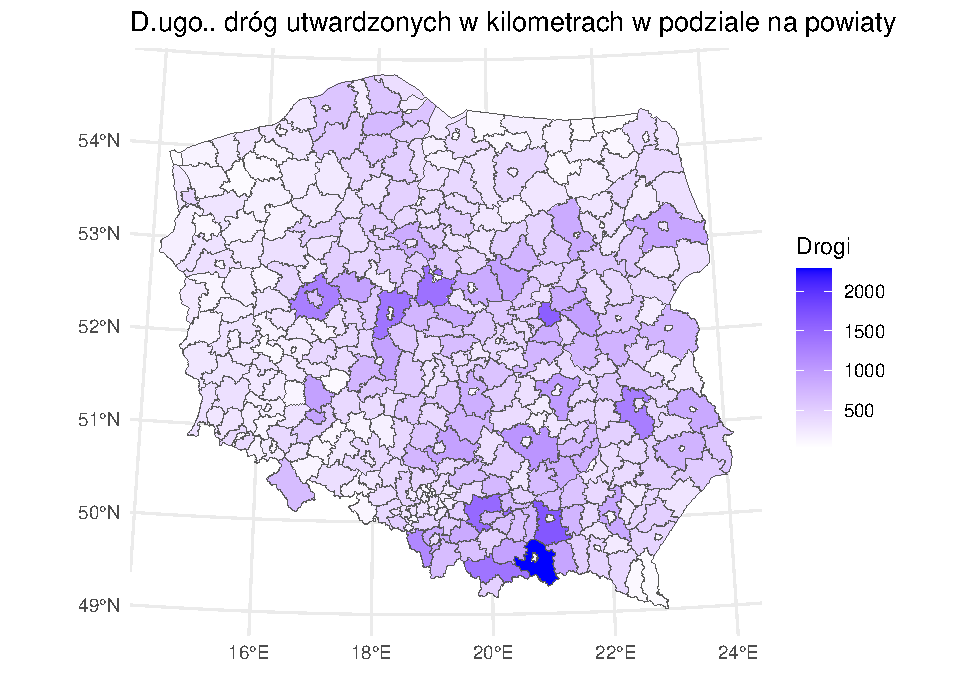
\includegraphics[keepaspectratio]{analiza_zanieczyszczenia_files/figure-latex/kart1-1.pdf}}

\pandocbounded{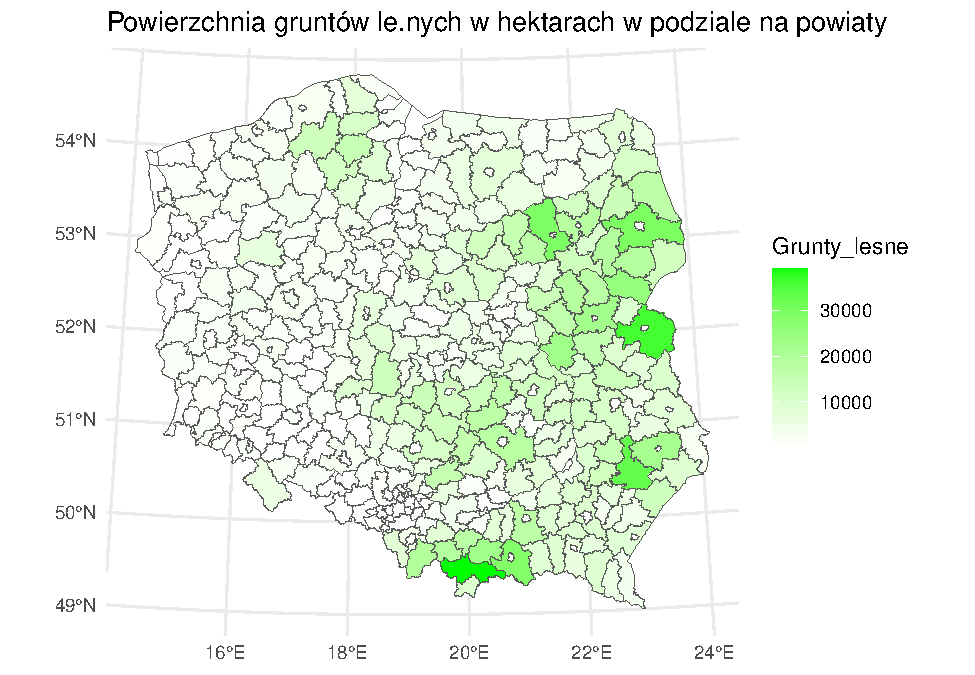
\includegraphics[keepaspectratio]{analiza_zanieczyszczenia_files/figure-latex/karrt2-1.pdf}}

\pandocbounded{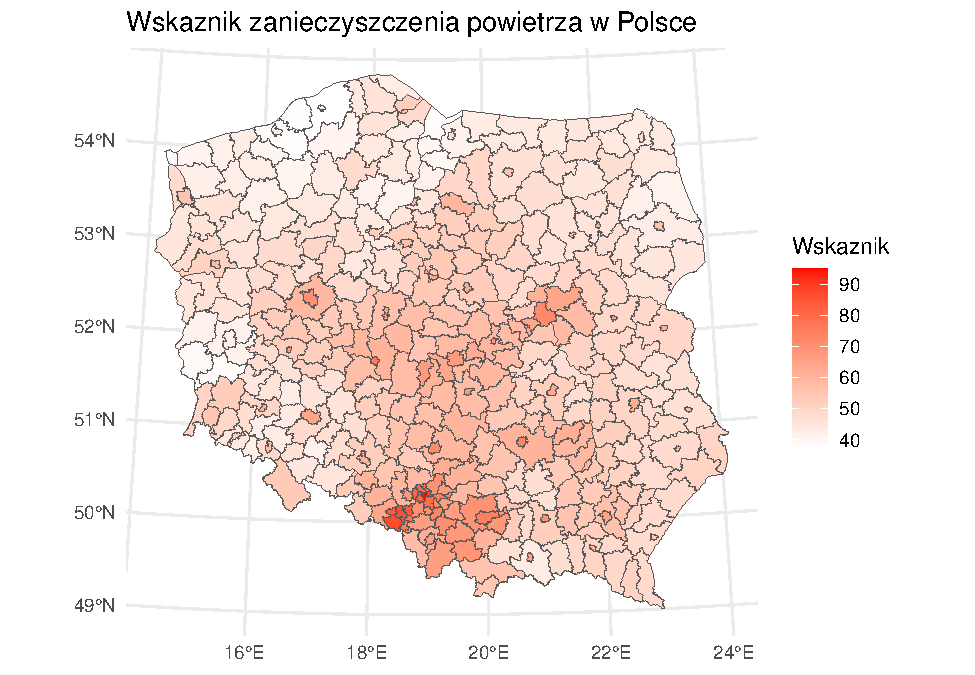
\includegraphics[keepaspectratio]{analiza_zanieczyszczenia_files/figure-latex/hji-1.pdf}}

\subsubsection{Kartogramy --
interpretacja}\label{kartogramy-interpretacja}

\begin{itemize}
\item
  \textbf{Zanieczyszczenie powietrza} w 2023 roku ma zróżnicowane
  rozmieszczenie, z wyższymi wartościami w południowej Polsce --
  szczególnie na Śląsku, co może wynikać z gęstej zabudowy i przemysłu.
\item
  \textbf{Długość dróg utwardzonych} również koncentruje się w regionach
  zurbanizowanych -- największe wartości widoczne są w aglomeracji
  śląskiej oraz okolicach dużych miast.
\item
  \textbf{Grunty leśne} dominują natomiast we wschodnich i
  południowo-wschodnich powiatach, gdzie przemysł i zaludnienie są
  mniejsze.
\end{itemize}

Rozkłady te wskazują na potencjalną zależność między środowiskiem,
infrastrukturą a zanieczyszczeniem -- co potwierdzają wcześniejsze
analizy korelacyjne i regresyjne.

\section{Analiza przestrzenna}\label{analiza-przestrzenna}

\begin{Shaded}
\begin{Highlighting}[]
\DocumentationTok{\#\#Identyfikacja przestrzennych skupisk i obserwacji odstających (hot/cold spots)}
\CommentTok{\# Moran I test}
\FunctionTok{moran.test}\NormalTok{(Dane}\SpecialCharTok{$}\NormalTok{Wskaznik, lw)}
\end{Highlighting}
\end{Shaded}

\begin{verbatim}
## 
##  Moran I test under randomisation
## 
## data:  Dane$Wskaznik  
## weights: lw    
## 
## Moran I statistic standard deviate = 21.693, p-value < 2.2e-16
## alternative hypothesis: greater
## sample estimates:
## Moran I statistic       Expectation          Variance 
##       0.733864665      -0.002638522       0.001152646
\end{verbatim}

\pandocbounded{\includegraphics[keepaspectratio]{analiza_zanieczyszczenia_files/figure-latex/moran2-1.pdf}}

Wartość statystyki Morana I wynosi \textbf{0.73} przy bardzo niskim
poziomie istotności (\emph{p} \textless{} 2.2e-16), co jednoznacznie
wskazuje na \textbf{silną i istotną przestrzenną autokorelację}
wskaźnika zanieczyszczenia powietrza. Oznacza to, że powiaty o podobnym
poziomie zanieczyszczenia tworzą przestrzenne klastry -- sąsiadujące
jednostki mają zbliżone wartości.

Wykres Morana (scatterplot) potwierdza ten wynik: dane dobrze układają
się wzdłuż rosnącej linii regresji, szczególnie w prawym górnym i lewym
dolnym ćwiartku, co oznacza obecność \textbf{hot i cold spotów} --
skupisk wysokich i niskich wartości.

\subsection{Mapa klastrów (hot/cold
spots)}\label{mapa-klastruxf3w-hotcold-spots}

\pandocbounded{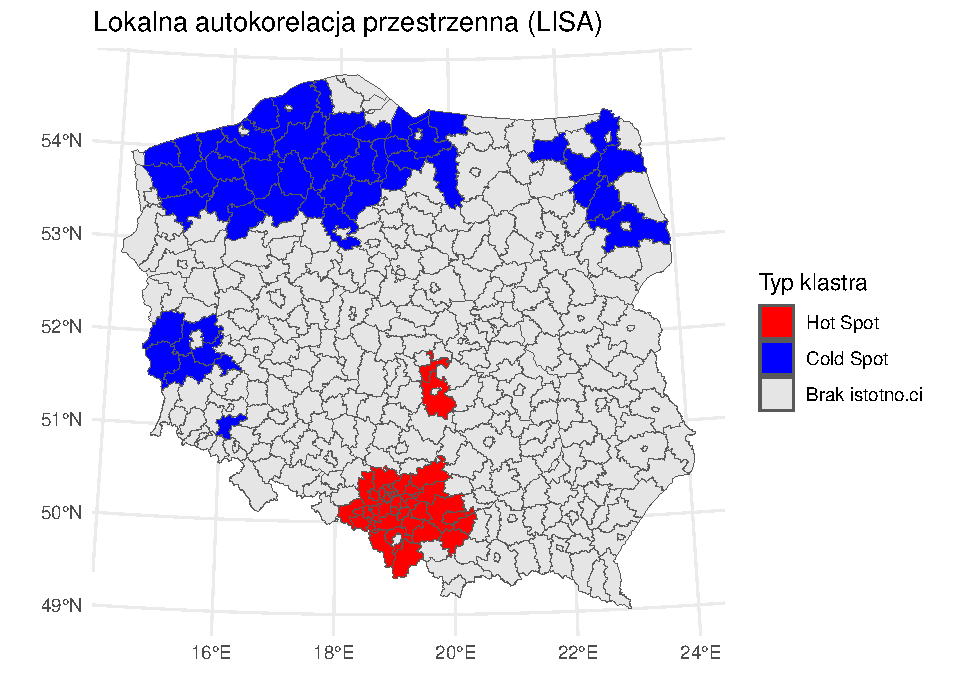
\includegraphics[keepaspectratio]{analiza_zanieczyszczenia_files/figure-latex/klas-1.pdf}}

Analiza lokalnej autokorelacji przestrzennej (LISA) ujawnia wyraźne
\textbf{klastry zanieczyszczenia powietrza}:

\begin{itemize}
\item
  \textbf{Hot spoty} (na czerwono) zlokalizowane są głównie na południu
  Polski, w tym na Śląsku -- obszarze o wysokim uprzemysłowieniu i
  gęstej zabudowie.
\item
  \textbf{Cold spoty} (na niebiesko) występują głównie w północnej i
  północno-wschodniej Polsce, co wskazuje na większy udział terenów
  zielonych i niższą gęstość zaludnienia.
\item
  Większość powiatów (na szaro) nie wykazuje istotnej lokalnej
  autokorelacji, co sugeruje zróżnicowanie wewnętrzne lub brak wyraźnych
  sąsiednich zależności.
\end{itemize}

Mapa potwierdza istnienie przestrzennych wzorców zanieczyszczenia, które
powinny być uwzględniane w politykach regionalnych.

\begin{Shaded}
\begin{Highlighting}[]
\CommentTok{\#Pomocniczy model liniowy}
\NormalTok{model\_stat }\OtherTok{\textless{}{-}} \FunctionTok{lm}\NormalTok{(}
\NormalTok{  Wskaznik }\SpecialCharTok{\textasciitilde{}}\NormalTok{ Liczba\_pojazdów }\SpecialCharTok{+}
\NormalTok{    Gm\_tereny\_zieleni }\SpecialCharTok{+}
\NormalTok{    Grunty\_lesne }\SpecialCharTok{+}
\NormalTok{    Pow\_powiatu }\SpecialCharTok{+}
\NormalTok{    Ludność\_na\_km2 }\SpecialCharTok{+}
\NormalTok{    Srednie\_wyn }\SpecialCharTok{+}
\NormalTok{    Drogi,}
  \AttributeTok{data =}\NormalTok{ Dane)}

\FunctionTok{summary}\NormalTok{(model\_stat)}
\end{Highlighting}
\end{Shaded}

\begin{verbatim}
## 
## Call:
## lm(formula = Wskaznik ~ Liczba_pojazdów + Gm_tereny_zieleni + 
##     Grunty_lesne + Pow_powiatu + Ludność_na_km2 + Srednie_wyn + 
##     Drogi, data = Dane)
## 
## Residuals:
##      Min       1Q   Median       3Q      Max 
## -24.9542  -3.6794  -0.4726   3.9080  27.7938 
## 
## Coefficients:
##                     Estimate Std. Error t value Pr(>|t|)    
## (Intercept)        5.727e+01  3.273e+00  17.495  < 2e-16 ***
## Liczba_pojazdów   -7.948e-06  4.432e-06  -1.793   0.0737 .  
## Gm_tereny_zieleni  1.278e+00  8.531e-01   1.498   0.1350    
## Grunty_lesne       1.069e-04  7.404e-05   1.444   0.1495    
## Pow_powiatu       -7.575e-05  1.008e-05  -7.517 4.23e-13 ***
## Ludność_na_km2     6.874e-03  1.372e-03   5.010 8.45e-07 ***
## Srednie_wyn       -7.302e-04  4.714e-04  -1.549   0.1222    
## Drogi              1.042e-02  1.714e-03   6.080 2.98e-09 ***
## ---
## Signif. codes:  0 '***' 0.001 '**' 0.01 '*' 0.05 '.' 0.1 ' ' 1
## 
## Residual standard error: 6.83 on 372 degrees of freedom
## Multiple R-squared:  0.5179, Adjusted R-squared:  0.5088 
## F-statistic: 57.09 on 7 and 372 DF,  p-value: < 2.2e-16
\end{verbatim}

Oszacowany model regresji tłumaczy około 52\% zmienności wskaźnika
zanieczyszczenia, co wskazuje na umiarkowaną trafność wyjaśniającą.
Istotny wpływ mają trzy zmienne: większa powierzchnia powiatu obniża
poziom zanieczyszczenia, natomiast większa gęstość zaludnienia i długość
dróg przyczyniają się do jego wzrostu. Pozostałe zmienne -- takie jak
liczba pojazdów, tereny zieleni czy wynagrodzenia -- mimo że mają
intuicyjny kierunek wpływu, nie są statystycznie istotne w tym modelu.
Model dobrze nadaje się jako baza do dalszej analizy, w tym rozbudowy o
komponent przestrzenny.

\section{Modelowanie ekonometryczne i ocena
modelu}\label{modelowanie-ekonometryczne-i-ocena-modelu}

\subsection{Model OLS}\label{model-ols}

\begin{Shaded}
\begin{Highlighting}[]
\CommentTok{\# Klasyczny model liniowy OLS}
\NormalTok{model\_ols }\OtherTok{\textless{}{-}} \FunctionTok{lm}\NormalTok{(Wskaznik }\SpecialCharTok{\textasciitilde{}}\NormalTok{ Liczba\_pojazdów }\SpecialCharTok{+}
\NormalTok{                  Gm\_tereny\_zieleni }\SpecialCharTok{+}
\NormalTok{                  Grunty\_lesne }\SpecialCharTok{+}
\NormalTok{                  Pow\_powiatu }\SpecialCharTok{+}
\NormalTok{                  Ludność\_na\_km2 }\SpecialCharTok{+}
\NormalTok{                  Srednie\_wyn }\SpecialCharTok{+}
\NormalTok{                  Drogi,}
                \AttributeTok{data =}\NormalTok{ Dane\_std)}
\CommentTok{\# Podsumowanie wyników}
\FunctionTok{summary}\NormalTok{(model\_ols)}
\end{Highlighting}
\end{Shaded}

\begin{verbatim}
## 
## Call:
## lm(formula = Wskaznik ~ Liczba_pojazdów + Gm_tereny_zieleni + 
##     Grunty_lesne + Pow_powiatu + Ludność_na_km2 + Srednie_wyn + 
##     Drogi, data = Dane_std)
## 
## Residuals:
##      Min       1Q   Median       3Q      Max 
## -2.56072 -0.37756 -0.04849  0.40102  2.85211 
## 
## Coefficients:
##                     Estimate Std. Error t value Pr(>|t|)    
## (Intercept)        8.222e-16  3.595e-02   0.000   1.0000    
## Liczba_pojazdów   -9.582e-02  5.343e-02  -1.793   0.0737 .  
## Gm_tereny_zieleni  1.111e-01  7.416e-02   1.498   0.1350    
## Grunty_lesne       6.807e-02  4.713e-02   1.444   0.1495    
## Pow_powiatu       -4.033e-01  5.365e-02  -7.517 4.23e-13 ***
## Ludność_na_km2     4.319e-01  8.622e-02   5.010 8.45e-07 ***
## Srednie_wyn       -6.287e-02  4.058e-02  -1.549   0.1222    
## Drogi              3.062e-01  5.036e-02   6.080 2.98e-09 ***
## ---
## Signif. codes:  0 '***' 0.001 '**' 0.01 '*' 0.05 '.' 0.1 ' ' 1
## 
## Residual standard error: 0.7008 on 372 degrees of freedom
## Multiple R-squared:  0.5179, Adjusted R-squared:  0.5088 
## F-statistic: 57.09 on 7 and 372 DF,  p-value: < 2.2e-16
\end{verbatim}

\begin{Shaded}
\begin{Highlighting}[]
\NormalTok{res\_squared }\OtherTok{\textless{}{-}} \FunctionTok{residuals}\NormalTok{(model\_ols)}\SpecialCharTok{\^{}}\DecValTok{2}
\FunctionTok{moran.test}\NormalTok{(res\_squared, lw)}
\end{Highlighting}
\end{Shaded}

\begin{verbatim}
## 
##  Moran I test under randomisation
## 
## data:  res_squared  
## weights: lw    
## 
## Moran I statistic standard deviate = 10.557, p-value < 2.2e-16
## alternative hypothesis: greater
## sample estimates:
## Moran I statistic       Expectation          Variance 
##       0.342511554      -0.002638522       0.001068803
\end{verbatim}

Model OLS wykazuje umiarkowane dopasowanie (R² ≈ 0.52), jednak test
Morana I dla reszt (I = 0.34, \emph{p} \textless{} 2.2e‑16) wskazuje na
istotną przestrzenną autokorelację, co sugeruje, że klasyczna regresja
nie uwzględnia zależności przestrzennych między powiatami. Współczynniki
regresji są zgodne z intuicją: większa powierzchnia powiatu i tereny
zieleni obniżają zanieczyszczenie, podczas gdy gęstość zaludnienia i
liczba pojazdów je zwiększają. Jednakże, brak istotności statystycznej
dla wielu zmiennych sugeruje potrzebę zastosowania bardziej
zaawansowanego modelowania przestrzennego.

\subsection{Model SAR (Spatial Autoregressive
Model)}\label{model-sar-spatial-autoregressive-model}

\begin{Shaded}
\begin{Highlighting}[]
\CommentTok{\# Spatial lag model (SAR)}
\CommentTok{\#Model SAR}
\NormalTok{model\_sar }\OtherTok{\textless{}{-}} \FunctionTok{lagsarlm}\NormalTok{(Wskaznik }\SpecialCharTok{\textasciitilde{}}\NormalTok{ Liczba\_pojazdów }\SpecialCharTok{+}
\NormalTok{                        Gm\_tereny\_zieleni }\SpecialCharTok{+}
\NormalTok{                        Grunty\_lesne }\SpecialCharTok{+}
\NormalTok{                        Pow\_powiatu }\SpecialCharTok{+}
\NormalTok{                        Ludność\_na\_km2 }\SpecialCharTok{+}
\NormalTok{                        Srednie\_wyn }\SpecialCharTok{+}
\NormalTok{                        Drogi,}
                      \AttributeTok{data =}\NormalTok{ mapa\_dane\_std,}\AttributeTok{listw =}\NormalTok{ lw, }\AttributeTok{method =} \StringTok{"eigen"}\NormalTok{, }\AttributeTok{zero.policy =} \ConstantTok{TRUE}\NormalTok{)}

\CommentTok{\# Podsumowanie wyników}
\FunctionTok{summary}\NormalTok{(model\_sar)}
\end{Highlighting}
\end{Shaded}

\begin{verbatim}
## 
## Call:lagsarlm(formula = Wskaznik ~ Liczba_pojazdów + Gm_tereny_zieleni + 
##     Grunty_lesne + Pow_powiatu + Ludność_na_km2 + Srednie_wyn + 
##     Drogi, data = mapa_dane_std, listw = lw, method = "eigen", 
##     zero.policy = TRUE)
## 
## Residuals:
##       Min        1Q    Median        3Q       Max 
## -1.142568 -0.186299 -0.023356  0.176798  1.220844 
## 
## Type: lag 
## Coefficients: (asymptotic standard errors) 
##                    Estimate Std. Error z value  Pr(>|z|)
## (Intercept)        0.077200   0.017311  4.4595 8.214e-06
## Liczba_pojazdów   -0.016513   0.025948 -0.6364 0.5245117
## Gm_tereny_zieleni -0.051163   0.035834 -1.4278 0.1533522
## Grunty_lesne       0.006162   0.022690  0.2716 0.7859466
## Pow_powiatu       -0.091473   0.026706 -3.4252 0.0006144
## Ludność_na_km2     0.410556   0.041604  9.8682 < 2.2e-16
## Srednie_wyn       -0.034431   0.019519 -1.7640 0.0777316
## Drogi              0.047296   0.025244  1.8735 0.0609950
## 
## Rho: 0.80325, LR test value: 484.12, p-value: < 2.22e-16
## Asymptotic standard error: 0.02118
##     z-value: 37.924, p-value: < 2.22e-16
## Wald statistic: 1438.3, p-value: < 2.22e-16
## 
## Log likelihood: -158.0098 for lag model
## ML residual variance (sigma squared): 0.11357, (sigma: 0.337)
## Number of observations: 380 
## Number of parameters estimated: 10 
## AIC: 336.02, (AIC for lm: 818.14)
## LM test for residual autocorrelation
## test value: 5.0144, p-value: 0.025137
\end{verbatim}

\begin{Shaded}
\begin{Highlighting}[]
\NormalTok{res\_squared1 }\OtherTok{\textless{}{-}} \FunctionTok{residuals}\NormalTok{(model\_sar)}\SpecialCharTok{\^{}}\DecValTok{2}
\FunctionTok{moran.test}\NormalTok{(res\_squared1, lw)}
\end{Highlighting}
\end{Shaded}

\begin{verbatim}
## 
##  Moran I test under randomisation
## 
## data:  res_squared1  
## weights: lw    
## 
## Moran I statistic standard deviate = 7.0816, p-value = 7.126e-13
## alternative hypothesis: greater
## sample estimates:
## Moran I statistic       Expectation          Variance 
##       0.233157637      -0.002638522       0.001108697
\end{verbatim}

Początkowy model liniowy wykazywał dobrą dopasowalność (R² ≈ 0.52),
jednak test Morana I dla reszt (I = 0.34, \emph{p} \textless{} 2.2e‑16)
ujawnił \textbf{istotną przestrzenną autokorelację}, co oznacza, że
klasyczna regresja niedoszacowuje wpływu zależności przestrzennych
między powiatami. W odpowiedzi zastosowano przestrzenny model SAR
(lagowy), który znacząco poprawił dopasowanie: wartość log-likelihood
wzrosła, a AIC spadło z 818 do 336, co potwierdza wyższość modelu
przestrzennego.

W modelu SAR współczynnik rho wynoszący 0.80 (istotny statystycznie)
wskazuje na silny przestrzenny efekt zależności między powiatami --
poziom zanieczyszczenia w jednym powiecie jest silnie powiązany ze
średnią w otoczeniu. Kluczowe zmienne, takie jak \textbf{gęstość
zaludnienia} i \textbf{powierzchnia powiatu}, pozostały istotne,
natomiast znaczenie innych predyktorów (np. liczby pojazdów, dróg)
osłabło po uwzględnieniu zależności przestrzennej.

Ostatecznie, także reszty z modelu SAR wykazują słabszą autokorelację
(Moran I = 0.23), co świadczy o lepszym uchwyceniu struktury danych.
Model SAR można uznać za trafniejsze narzędzie analizy regionalnych
różnic w zanieczyszczeniu powietrza.

\subsection{Model SEM}\label{model-sem}

\begin{Shaded}
\begin{Highlighting}[]
\NormalTok{sem\_model }\OtherTok{\textless{}{-}} \FunctionTok{spautolm}\NormalTok{(}
  \AttributeTok{formula =}\NormalTok{ Wskaznik }\SpecialCharTok{\textasciitilde{}}\NormalTok{ Liczba\_pojazdów }\SpecialCharTok{+}\NormalTok{ Pow\_powiatu }\SpecialCharTok{+}\NormalTok{ Ludność\_na\_km2 }\SpecialCharTok{+}\NormalTok{ Drogi,}
  \AttributeTok{data =}\NormalTok{ Dane\_std,}
  \AttributeTok{listw =}\NormalTok{ lw,  }\CommentTok{\# lub "b" w nowszych wersjach}
  \AttributeTok{method =} \StringTok{"eigen"}
\NormalTok{)}
\FunctionTok{summary}\NormalTok{(sem\_model)}
\end{Highlighting}
\end{Shaded}

\begin{verbatim}
## 
## Call: spautolm(formula = Wskaznik ~ Liczba_pojazdów + Pow_powiatu + 
##     Ludność_na_km2 + Drogi, data = Dane_std, listw = lw, method = "eigen")
## 
## Residuals:
##      Min       1Q   Median       3Q      Max 
## -0.79150 -0.19493 -0.03304  0.15692  1.27682 
## 
## Coefficients: 
##                   Estimate Std. Error z value Pr(>|z|)
## (Intercept)      0.0321753  0.2625946  0.1225  0.90248
## Liczba_pojazdów -0.0601730  0.0247191 -2.4343  0.01492
## Pow_powiatu      0.0245073  0.0266622  0.9192  0.35800
## Ludność_na_km2   0.4430950  0.0327530 13.5284  < 2e-16
## Drogi           -0.0077158  0.0247355 -0.3119  0.75509
## 
## Lambda: 0.93295 LR test value: 469.9 p-value: < 2.22e-16 
## Numerical Hessian standard error of lambda: 0.017963 
## 
## Log likelihood: -168.3819 
## ML residual variance (sigma squared): 0.10818, (sigma: 0.32891)
## Number of observations: 380 
## Number of parameters estimated: 7 
## AIC: 350.76
\end{verbatim}

\begin{Shaded}
\begin{Highlighting}[]
\NormalTok{res\_squared2 }\OtherTok{\textless{}{-}} \FunctionTok{residuals}\NormalTok{(sem\_model)}\SpecialCharTok{\^{}}\DecValTok{2}
\FunctionTok{moran.test}\NormalTok{(res\_squared2, lw)}
\end{Highlighting}
\end{Shaded}

\begin{verbatim}
## 
##  Moran I test under randomisation
## 
## data:  res_squared2  
## weights: lw    
## 
## Moran I statistic standard deviate = 6.3017, p-value = 1.472e-10
## alternative hypothesis: greater
## sample estimates:
## Moran I statistic       Expectation          Variance 
##       0.205775536      -0.002638522       0.001093796
\end{verbatim}

Model przestrzenny SAR z istotnym współczynnikiem lambda (0.93, \emph{p}
\textless{} 2.2e‑16) potwierdza silną zależność przestrzenną między
powiatami -- zanieczyszczenie w jednym regionie jest silnie skorelowane
z jego otoczeniem. W porównaniu do regresji klasycznej, model ten lepiej
dopasowuje się do danych (niższy AIC = 350, wyższy log-likelihood).

Wśród zmiennych objaśniających tylko \textbf{ludność na km²} (\emph{p}
\textless{} 2e‑16) i w mniejszym stopniu \textbf{liczba pojazdów}
(\emph{p} ≈ 0.015) wykazują istotny wpływ. Natomiast
\textbf{powierzchnia powiatu} i \textbf{długość dróg} nie są
statystycznie znaczące po uwzględnieniu zależności przestrzennych.

Test Morana I wykonany dla reszt modelu SAR wskazuje, że autokorelacja
została istotnie zredukowana (\emph{I} = 0.21, \emph{p} \textless{}
0.001), co potwierdza poprawność specyfikacji modelu przestrzennego i
jego przewagę nad klasyczną regresją.

\subsection{Przestrzenny Model Durbina
(SDM)}\label{przestrzenny-model-durbina-sdm}

\begin{Shaded}
\begin{Highlighting}[]
\NormalTok{sdm\_model }\OtherTok{\textless{}{-}} \FunctionTok{lagsarlm}\NormalTok{(}
  \AttributeTok{formula =}\NormalTok{ Wskaznik }\SpecialCharTok{\textasciitilde{}}\NormalTok{ Liczba\_pojazdów }\SpecialCharTok{+}
\NormalTok{    Pow\_powiatu }\SpecialCharTok{+}
\NormalTok{    Ludność\_na\_km2 }\SpecialCharTok{+}
\NormalTok{    Drogi,}
    \AttributeTok{data =}\NormalTok{ Dane\_std,}
  \AttributeTok{listw =}\NormalTok{ lw,}
  \AttributeTok{Durbin =} \ConstantTok{TRUE}
\NormalTok{)}

\FunctionTok{summary}\NormalTok{(sdm\_model)}
\end{Highlighting}
\end{Shaded}

\begin{verbatim}
## 
## Call:lagsarlm(formula = Wskaznik ~ Liczba_pojazdów + Pow_powiatu + 
##     Ludność_na_km2 + Drogi, data = Dane_std, listw = lw, Durbin = TRUE)
## 
## Residuals:
##       Min        1Q    Median        3Q       Max 
## -1.035137 -0.200038 -0.016297  0.178699  1.269908 
## 
## Type: mixed 
## Coefficients: (asymptotic standard errors) 
##                      Estimate Std. Error z value  Pr(>|z|)
## (Intercept)          0.040883   0.020057  2.0384  0.041509
## Liczba_pojazdów     -0.046804   0.025835 -1.8117  0.070037
## Pow_powiatu         -0.021513   0.028605 -0.7521  0.451998
## Ludność_na_km2       0.419540   0.033027 12.7028 < 2.2e-16
## Drogi                0.013649   0.026785  0.5096  0.610350
## lag.Liczba_pojazdów  0.031304   0.044197  0.7083  0.478768
## lag.Pow_powiatu     -0.072388   0.034743 -2.0835  0.037202
## lag.Ludność_na_km2  -0.205120   0.067172 -3.0537  0.002261
## lag.Drogi            0.069231   0.029937  2.3125  0.020748
## 
## Rho: 0.84412, LR test value: 347.08, p-value: < 2.22e-16
## Asymptotic standard error: 0.02783
##     z-value: 30.331, p-value: < 2.22e-16
## Wald statistic: 919.98, p-value: < 2.22e-16
## 
## Log likelihood: -150.0565 for mixed model
## ML residual variance (sigma squared): 0.1061, (sigma: 0.32573)
## Number of observations: 380 
## Number of parameters estimated: 11 
## AIC: 322.11, (AIC for lm: 667.19)
## LM test for residual autocorrelation
## test value: 1.8766, p-value: 0.17072
\end{verbatim}

\begin{Shaded}
\begin{Highlighting}[]
\NormalTok{res\_squared3 }\OtherTok{\textless{}{-}} \FunctionTok{residuals}\NormalTok{(sdm\_model)}\SpecialCharTok{\^{}}\DecValTok{2}
\FunctionTok{moran.test}\NormalTok{(res\_squared3, lw)}
\end{Highlighting}
\end{Shaded}

\begin{verbatim}
## 
##  Moran I test under randomisation
## 
## data:  res_squared3  
## weights: lw    
## 
## Moran I statistic standard deviate = 6.6705, p-value = 1.274e-11
## alternative hypothesis: greater
## sample estimates:
## Moran I statistic       Expectation          Variance 
##       0.218166821      -0.002638522       0.001095713
\end{verbatim}

Model SAR z komponentem Durbin (efekty sąsiedztwa w zmiennych
niezależnych) charakteryzuje się bardzo dobrym dopasowaniem (AIC = 322,
log-likelihood = --150), znacznie lepszym niż klasyczna regresja liniowa
(AIC = 667). Współczynnik rho = 0.84 (istotny przy \emph{p} \textless{}
2.2e-16) potwierdza silną autokorelację przestrzenną w poziomie
zanieczyszczenia.

Najważniejsze obserwacje:

\begin{itemize}
\item
  \textbf{Ludność na km²} pozostaje silnie i istotnie dodatnio związana
  z poziomem zanieczyszczenia (\emph{p} \textless{} 2e-16),
\item
  Efekty przestrzenne (sąsiedztwa) są istotne w przypadku:

  \begin{itemize}
  \item
    \textbf{Lag.Pow\_powiatu} (\emph{p} = 0.037) -- większe sąsiednie
    powiaty obniżają zanieczyszczenie,
  \item
    \textbf{Lag.Ludność\_na\_km²} (\emph{p} = 0.002) -- otoczenie o
    dużej gęstości ludności zwiększa zanieczyszczenie,
  \item
    \textbf{Lag.Drogi} (\emph{p} = 0.020) -- wpływ infrastruktury
    sąsiadujących powiatów także jest pozytywny.
  \end{itemize}
\end{itemize}

Model Durbin lepiej oddaje złożoną zależność przestrzenną, gdzie nie
tylko lokalne, ale też sąsiednie warunki mają wpływ na jakość powietrza.
Test Morana I dla reszt wskazuje, że choć pewna autokorelacja pozostaje
(\emph{I} ≈ 0.22), to została znacznie zredukowana względem modelu
klasycznego.

\textbf{Podsumowanie}

Zastosowanie metod ekonometrii przestrzennej w analizie zanieczyszczenia
powietrza było uzasadnione charakterem badanego zjawiska. Przeprowadzone
testy autokorelacji przestrzennej, w tym test Morana I, potwierdziły
istnienie istotnych statystycznie zależności przestrzennych w rozkładzie
wskaźnika zanieczyszczeń.

Wykorzystanie różnych specyfikacji modeli przestrzennych (SLX, SEM, SAR,
SDM) pozwoliło na kompleksową analizę mechanizmów przestrzennego
oddziaływania. Model SLX (Spatial Lag of X) uwzględnia przestrzenne
opóźnienia zmiennych objaśniających, co jest szczególnie istotne w
kontekście efektów spillover infrastruktury drogowej czy emisji z
sąsiednich powiatów (Feng et al., 2020). Model SEM (Spatial Error Model)
kontroluje przestrzenną autokorelację w składniku losowym, która może
wynikać z pominiętych zmiennych o charakterze przestrzennym. Model SAR
(Spatial Autoregressive) bezpośrednio modeluje wpływ poziomu
zanieczyszczeń w sąsiednich powiatach, co odzwierciedla procesy dyfuzji
zanieczyszczeń. Najbardziej kompleksowy model SDM (Spatial Durbin Model)
łączy elementy SAR i SLX, umożliwiając jednoczesną analizę efektów
bezpośrednich, pośrednich i całkowitych (Elhorst, 2014).

\subsection{Model SLX (Spatial Lag of
X)}\label{model-slx-spatial-lag-of-x}

\begin{Shaded}
\begin{Highlighting}[]
\NormalTok{slx\_model }\OtherTok{\textless{}{-}} \FunctionTok{lmSLX}\NormalTok{(}
  \AttributeTok{formula =}\NormalTok{ Wskaznik }\SpecialCharTok{\textasciitilde{}}\NormalTok{ Liczba\_pojazdów }\SpecialCharTok{+}
\NormalTok{    Pow\_powiatu }\SpecialCharTok{+}
\NormalTok{    Ludność\_na\_km2 }\SpecialCharTok{+}
\NormalTok{    Drogi,}
  \AttributeTok{data =}\NormalTok{ Dane\_std,}
  \AttributeTok{listw =}\NormalTok{ lw}
\NormalTok{)}

\FunctionTok{summary}\NormalTok{(slx\_model)}
\end{Highlighting}
\end{Shaded}

\begin{verbatim}
## 
## Call:
## lm(formula = formula(paste("y ~ ", paste(colnames(x)[-1], collapse = "+"))), 
##     data = as.data.frame(x), weights = weights)
## 
## Coefficients:
##                      Estimate    Std. Error  t value     Pr(>|t|)  
## (Intercept)           1.905e-01   3.409e-02   5.588e+00   4.447e-08
## Liczba_pojazdów      -4.121e-02   4.551e-02  -9.053e-01   3.659e-01
## Pow_powiatu          -1.711e-01   4.977e-02  -3.437e+00   6.554e-04
## Ludność_na_km2        3.997e-01   5.817e-02   6.870e+00   2.718e-11
## Drogi                 7.895e-02   4.697e-02   1.681e+00   9.367e-02
## lag.Liczba_pojazdów  -1.915e-01   7.651e-02  -2.502e+00   1.277e-02
## lag.Pow_powiatu      -3.411e-01   5.896e-02  -5.785e+00   1.543e-08
## lag.Ludność_na_km2    6.486e-01   1.064e-01   6.097e+00   2.711e-09
## lag.Drogi             2.875e-01   4.972e-02   5.782e+00   1.567e-08
\end{verbatim}

\begin{Shaded}
\begin{Highlighting}[]
\NormalTok{res\_squared4 }\OtherTok{\textless{}{-}} \FunctionTok{residuals}\NormalTok{(slx\_model)}\SpecialCharTok{\^{}}\DecValTok{2}
\FunctionTok{moran.test}\NormalTok{(res\_squared4, lw)}
\end{Highlighting}
\end{Shaded}

\begin{verbatim}
## 
##  Moran I test under randomisation
## 
## data:  res_squared4  
## weights: lw    
## 
## Moran I statistic standard deviate = 12.873, p-value < 2.2e-16
## alternative hypothesis: greater
## sample estimates:
## Moran I statistic       Expectation          Variance 
##       0.414206198      -0.002638522       0.001048547
\end{verbatim}

Model regresji z efektami sąsiedztwa (zmienne opóźnione przestrzennie) i
wagami dostarcza mocnych dowodów na istotność zarówno lokalnych, jak i
otaczających czynników. Istotność przestrzenna została potwierdzona
przez test Morana I dla reszt (\emph{I} ≈ 0.41, \emph{p} \textless{}
2.2e-16), co sugeruje, że mimo zastosowanych wag, zależności
przestrzenne nadal są silne.

Wnioski z modelu:

\begin{itemize}
\item
  \textbf{Ludność na km²} (lokalnie i w otoczeniu) ma bardzo silny
  pozytywny wpływ -- zagęszczenie ludności silnie wiąże się z wyższym
  poziomem zanieczyszczenia.
\item
  \textbf{Powierzchnia powiatu} (zarówno lokalna, jak i sąsiedzka)
  działa w przeciwnym kierunku -- większe obszary wiążą się z niższym
  zanieczyszczeniem.
\item
  \textbf{Lag.Drogi} oraz \textbf{lag.Liczba\_pojazdów} również są
  istotne i dodatnie -- warunki infrastrukturalne w sąsiedztwie powiatu
  wzmacniają efekt zanieczyszczenia.
\end{itemize}

Model podkreśla znaczenie \textbf{rozszerzonego otoczenia
terytorialnego} -- jakość powietrza zależy nie tylko od warunków w danym
powiecie, ale również od tego, co dzieje się w jego sąsiedztwie.

\section{Wnioski}\label{wnioski}

Przeprowadzona analiza potwierdziła, że zanieczyszczenie powietrza w
Polsce ma wyraźny charakter przestrzenny -- wartości wskaźnika są silnie
powiązane nie tylko z cechami danego powiatu, ale także z sytuacją w
jego otoczeniu. Najlepsze dopasowanie uzyskano w modelu SDM (Spatial
Durbin Model), który uwzględnia zarówno lokalne predyktory, jak i efekt
sąsiedztwa (zmienne opóźnione przestrzennie).

Za najważniejszy czynnik uznano gęstość zaludnienia, która lokalnie
znacząco zwiększa poziom zanieczyszczenia, a jednocześnie -- w przypadku
sąsiednich powiatów -- może działać hamująco. Uwagę zwracają również
istotne przestrzenne efekty infrastruktury (drogi) i powierzchni
jednostek terytorialnych. Klasyczny model regresji (OLS) nie uwzględnia
tych zależności i prowadzi do błędnych wniosków -- co potwierdzają
silnie skorelowane reszty (Moran I ≈ 0.73).

W kontekście polityki publicznej oznacza to, że skuteczna strategia
poprawy jakości powietrza powinna być koordynowana regionalnie, a nie
ograniczać się do pojedynczych powiatów. Działania inwestycyjne i
planistyczne powinny być planowane z uwzględnieniem danych z otoczenia,
np. przez współpracę między powiatami w ramach subregionów
funkcjonalnych.

Należy jednak pamiętać o ograniczeniach: dane są przekrojowe,
zagregowane i mogą zawierać uproszczenia. Choć model SDM dobrze
odwzorowuje zależności przestrzenne, nie uwzględnia nieliniowości czy
lokalnych wariantów zależności.

Geograficznie Ważona Regresja (Geographically Weighted Regression - GWR)
stanowi naturalne rozszerzenie przeprowadzonych analiz i powinna być
rozważona w kolejnym etapie badań z następujących powodów:

Heterogeniczność przestrzenna: Polska charakteryzuje się znacznym
zróżnicowaniem regionalnym pod względem struktury gospodarczej, gęstości
zaludnienia i warunków klimatycznych. GWR umożliwi identyfikację
lokalnych wzorców determinant zanieczyszczenia powietrza, które mogą
różnić się między np. uprzemysłowionym Śląskiem a rolniczymi regionami
wschodniej Polski (Zhou et al., 2019).

Nieliniowość relacji przestrzennych: Metoda GWR pozwala na estymację
parametrów zmieniających się w przestrzeni, co jest szczególnie istotne
dla zmiennych takich jak wpływ terenów zielonych, który może być różny w
zależności od lokalnego kontekstu urbanistycznego (Fotheringham et al.,
2002).

Wsparcie polityki regionalnej: Lokalne oszacowania parametrów dostarczą
bardziej precyzyjnych informacji dla decydentów na poziomie powiatowym i
wojewódzkim, umożliwiając dostosowanie strategii redukcji zanieczyszczeń
do specyfiki danego regionu. Jak wykazali Lu et al.~(2014), dopasowanie
modelu GWR (mierzone R²) jest znacznie lepsze niż klasycznej regresji
OLS dla analiz zanieczyszczeń powietrza. Komplementarność z modelami
globalnymi: GWR nie zastępuje, lecz uzupełnia globalne modele
przestrzenne, dostarczając informacji o lokalnych odchyleniach od
średnich efektów oszacowanych w modelach SAR czy SDM (Wang et al.,
2019).

\section{Bibliografia}\label{bibliografia}

Abhijith, K. V., Kumar, P., Gallagher, J., McNabola, A., Baldauf, R.,
Pilla, F., \ldots{} \& Pulvirenti, B. (2017). Air pollution abatement
performances of green infrastructure in open road and built-up street
canyon environments--A review. Atmospheric Environment, 162, 71-86.

Balun, M., Białoskórska, U., Bruszewski, H., Burzyński, J., Błaszczyk,
J., Cenowski, M., \ldots{} \& Hławiczka, S. (2011). Analiza stanu
zanieczyszczenia powietrza pyłem PM10 i PM2,5 z uwzględnieniem składu
chemicznego pyłu oraz wpływu źródeł naturalnych---Raport końcowy.
Instytut Podstaw Inżynierii Środowiska PAN.

Chen, L., Liu, C., Zhang, L., Zou, R., \& Zhang, Z. (2023). The impact
of greenspace on air pollution: Empirical evidence from China.
Ecological Indicators, 146, 109881.

Cheng, Z., Pang, M. S., \& Pavlou, P. A. (2020). Mitigating traffic
congestion: The role of intelligent transportation systems. Information
Systems Research, 31(3), 653-674.

Elhorst, J. P. (2014). Spatial econometrics: From cross-sectional data
to spatial panels. Springer.

Feng, T., Du, H., Lin, Z., \& Zuo, J. (2020). Spatial spillover effects
of environmental regulations on air pollution: Evidence from urban
agglomerations in China. Journal of Environmental Management, 272,
110998.

Fotheringham, A. S., Brunsdon, C., \& Charlton, M. (2002).
Geographically weighted regression: The analysis of spatially varying
relationships. John Wiley \& Sons. Holnicki, P., Tainio, M., Kałuszko,
A., \& Nahorski, Z. (2018). Burden of disease due to air pollution in
Warsaw, Poland. International Journal of Environmental Research and
Public Health, 15(9), 1-16.

Kumar, P., Druckman, A., Gallagher, J., Gatersleben, B., Allison, S.,
Eisenman, T. S., \ldots{} \& Morawska, L. (2024). Reassessing the role
of urban green space in air pollution control. Proceedings of the
National Academy of Sciences, 121(3), e2306200121.

Lou, C. R., Liu, H. Y., Li, Y. F., \& Li, Y. L. (2021). Socioeconomic
drivers of PM2.5 in the accumulation phase of air pollution: A regional
analysis of 254 Chinese cities. International Journal of Environmental
Research and Public Health, 18(17), 9019.

Lu, D., Xu, J., Yang, D., \& Zhao, J. (2014). Spatio-temporal variation
and influence factors of PM2.5 concentrations in China from 1998 to
2014. Atmospheric Pollution Research, 8(6), 1151-1159.

Maciejewska, M. (2020). Short-term impact of PM2.5, PM10, and PMc on
mortality and morbidity in the agglomeration of Warsaw, Poland. Air
Quality, Atmosphere \& Health, 13(6), 659-672.

Wang, Y., Huang, B., \& Yang, L. (2019). A geographically and temporally
weighted regression model for spatial downscaling of MODIS land surface
temperatures over urban heterogeneous regions. IEEE Transactions on
Geoscience and Remote Sensing, 57(7), 5012-5027.

Zhang, X., You, C., \& Chen, S. (2024). Road traffic infrastructure
construction and air pollution based on the perspective of spatial
spillover. Sustainability, 16(21), 9627.

Zhou, Q., Wang, C., \& Fang, S. (2019). Application of geographically
weighted regression (GWR) in the analysis of the cause of haze pollution
in China. Atmospheric Pollution Research, 10(3), 835-846.

\end{document}
